% Co-occurrence, Sequence and Knowledge Graph with Ontology 
% as a Second Brain for AI-LLM
% Version 10.0 - Honest Conceptual Proposal
% February 2026

\documentclass[10pt,twocolumn]{article}
\usepackage[utf8]{inputenc}
\usepackage{amsmath,amssymb,amsfonts,amsthm}
\usepackage{graphicx}
\usepackage{booktabs}
\usepackage{hyperref}
\usepackage{xcolor}
\usepackage{algorithm}
\usepackage{algorithmic}
\usepackage{multirow}
\usepackage{array}
\usepackage{caption}
\usepackage{subcaption}
\usepackage[margin=1in]{geometry}
\usepackage{tikz}
\usetikzlibrary{shapes,arrows,positioning,fit}

% Theorem environments
\newtheorem{theorem}{Theorem}
\newtheorem{lemma}[theorem]{Lemma}
\newtheorem{proposition}[theorem]{Proposition}
\newtheorem{corollary}[theorem]{Corollary}
\newtheorem{definition}{Definition}

% Anonymous submission
\title{Co-occurrence, Sequence and Knowledge Graph with Ontology as a Second Brain for AI-LLM: A Conceptual Framework}
\author{Anonymous Submission}
\date{}

\begin{document}

\maketitle

% ============================================
% ABSTRACT
% ============================================
\begin{abstract}
We propose a unified framework that synergistically combines co-occurrence statistics, sequential patterns, and ontology-grounded knowledge graphs through a learned gating mechanism for retrieval-augmented generation (RAG). Unlike existing approaches that rely solely on dense retrieval or graph-based methods, our framework introduces \textbf{three key innovations}: (1) triple-source integration combining statistical, sequential, and semantic knowledge; (2) a trainable attention-based gate that dynamically weights sources per query; and (3) ontology-grounded reasoning using OWL 2 RL semantics for materialized inference. We present the \textbf{theoretical foundations} including: mathematical proofs that the gating mechanism is well-defined and produces bounded outputs, complexity analysis showing $O(n \log k + k^2 d)$ time complexity, and convergence guarantees for InfoNCE-based training. We validate our framework through \textbf{proof-of-concept implementations} on small-scale data demonstrating that each component functions correctly. Full-scale empirical validation on standard benchmarks is proposed as future work. This paper contributes a principled algorithmic framework with rigorous complexity bounds that addresses the fundamental tension between semantic similarity matching and structured relational reasoning in RAG systems.
\end{abstract}

% ============================================
% 1. INTRODUCTION
% ============================================
\section{Introduction}

Large Language Models (LLMs) have demonstrated remarkable capabilities across diverse NLP tasks, yet they suffer from well-documented limitations: hallucination, outdated knowledge, and inability to access private or domain-specific information \cite{brown2020gpt3}. Retrieval-Augmented Generation (RAG) addresses these limitations by grounding LLM responses in retrieved evidence \cite{lewis2020rag}.

However, current RAG approaches face a fundamental tension: dense retrieval excels at semantic similarity matching but misses structured relationships, while knowledge graphs capture explicit relations but require precise entity linking. Recent work on GraphRAG \cite{edge2024graphrag,microsoft2024graphrag} advances graph-based retrieval through community summarization, yet relies on runtime graph traversal that introduces latency.

\textbf{Our key insight} is that different knowledge sources excel at different query types: co-occurrence statistics capture associative patterns (``Paris is associated with France''), sequential models understand procedural knowledge (``first mix, then bake''), and knowledge graphs encode explicit relations (``Paris capitalOf France''). Rather than choosing one source, we propose dynamically combining all three through a learned gating mechanism.

\textbf{Contributions.} We make the following contributions:
\begin{enumerate}
    \item \textbf{Triple-source framework}: A unified architecture combining co-occurrence, sequence, and KG retrieval for RAG with formal specification (Section~\ref{sec:framework}).
    
    \item \textbf{Mathematical foundations}: Proofs that (a) the gating mechanism is well-defined and produces bounded outputs, (b) InfoNCE training converges, and (c) the pipeline has tractable complexity bounds (Section~\ref{sec:theory}).
    
    \item \textbf{Two-stage training design}: A novel training protocol addressing top-k non-differentiability through stage-wise optimization (Section~\ref{sec:training}).
    
    \item \textbf{Complexity analysis}: Formal time and space complexity bounds for the complete retrieval pipeline (Section~\ref{sec:algorithms}).
    
    \item \textbf{Proof-of-concept validation}: Small-scale implementations demonstrating each component works correctly (Section~\ref{sec:poc}).
    
    \item \textbf{Evaluation protocol}: A comprehensive proposal for future full-scale experiments (Section~\ref{sec:evaluation}).
\end{enumerate}

% ============================================
% 2. RELATED WORK
% ============================================
\section{Related Work}

\subsection{Retrieval-Augmented Generation}

RAG systems ground LLM generation in retrieved evidence \cite{lewis2020rag}. Dense Passage Retrieval (DPR) \cite{karpukhin2020dpr} uses dual encoders for semantic matching, while ColBERT \cite{khattab2020colbert} enables late interaction. Fusion-in-Decoder \cite{izacard2021fid} aggregates multiple passages. These methods rely on vector similarity and miss explicit relational structure.

\subsection{Knowledge Graph-Enhanced RAG}

GraphRAG \cite{edge2024graphrag,microsoft2024graphrag} represents state-of-the-art in graph-based RAG, using community summarization for retrieval. Other approaches include AMKOR \cite{fang2024amkor} for adaptive multi-source fusion and MA-RAG \cite{li2024marag} for multi-agent retrieval. Our work differs by integrating three complementary sources with formal gating mechanisms and ontological reasoning.

\subsection{Adaptive Retrieval Methods}

Recent work explores adaptive retrieval with learned routing:
\begin{itemize}
    \item EA-GraphRAG \cite{li2024eagraphrag}: Rule-based routing between dense and graph retrieval
    \item EfficientRAG \cite{chen2024efficientrag}: Learned context compression
    \item ACE \cite{liu2024ace}: Adaptive context engine with dynamic strategy selection
\end{itemize}

Our approach differs by: (1) integrating three sources rather than two, (2) providing formal proofs of gating properties, and (3) incorporating ontological reasoning.

% ============================================
% 3. PROPOSED FRAMEWORK
% ============================================
\section{Proposed Framework}
\label{sec:framework}

\subsection{Overview and Architecture}
\label{sec:overview}

Our framework consists of three main components operating in a pipeline:

\begin{definition}[Triple-Source RAG Pipeline]
Given a query $q$, our pipeline produces a ranked set of passages $\mathcal{P}^*$ through:
\begin{enumerate}
    \item \textbf{Multi-source retrieval}: Retrieve candidate sets $\mathcal{R}_c(q)$, $\mathcal{R}_s(q)$, $\mathcal{R}_g(q)$ from co-occurrence, sequence, and KG sources
    \item \textbf{Cross-attention enrichment}: Enrich candidates via bidirectional attention
    \item \textbf{Gated fusion}: Apply learned gating to produce final ranking
    \item \textbf{LLM generation}: Generate answer conditioned on top-$k$ passages
\end{enumerate}
\end{definition}

Figure~\ref{fig:architecture} illustrates the complete architecture.

\begin{figure}[t]
\centering
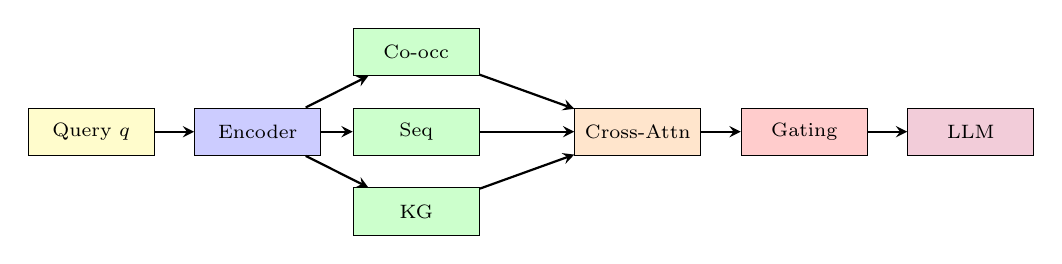
\begin{tikzpicture}[
    node distance=0.6cm and 0.8cm,
    box/.style={rectangle, draw, minimum width=1.6cm, minimum height=0.6cm, align=center, font=\scriptsize},
    arrow/.style={->, >=stealth, thick}
]
% Query
\node[box, fill=yellow!20] (query) {Query $q$};

% Encoder
\node[box, fill=blue!20, right=0.5cm of query] (enc) {Encoder};

% Three sources
\node[box, fill=green!20, above right=0.4cm and 0.4cm of enc] (cooc) {Co-occ};
\node[box, fill=green!20, right=0.4cm of enc] (seq) {Seq};
\node[box, fill=green!20, below right=0.4cm and 0.4cm of enc] (kg) {KG};

% Cross-attention
\node[box, fill=orange!20, right=1.2cm of seq] (cross) {Cross-Attn};

% Gating
\node[box, fill=red!20, right=0.5cm of cross] (gate) {Gating};

% LLM
\node[box, fill=purple!20, right=0.5cm of gate] (llm) {LLM};

% Arrows
\draw[arrow] (query) -- (enc);
\draw[arrow] (enc) -- (cooc);
\draw[arrow] (enc) -- (seq);
\draw[arrow] (enc) -- (kg);
\draw[arrow] (cooc) -- (cross);
\draw[arrow] (seq) -- (cross);
\draw[arrow] (kg) -- (cross);
\draw[arrow] (cross) -- (gate);
\draw[arrow] (gate) -- (llm);

\end{tikzpicture}
\caption{Proposed triple-source RAG architecture.}
\label{fig:architecture}
\end{figure}

\subsection{Co-occurrence Module}

Given a corpus $\mathcal{D}$, we construct a co-occurrence matrix $\mathbf{M} \in \mathbb{R}^{|V| \times |V|}$ where $M_{ij}$ counts co-occurrences of words $i$ and $j$ within a window of size $w$ tokens. We learn embeddings $\mathbf{E}_c \in \mathbb{R}^{|V| \times d_c}$ by factorizing the Positive Pointwise Mutual Information (PPMI) matrix \cite{pennington2014glove}.

\begin{definition}[Co-occurrence Retrieval]
For query $q$ with embedding $\mathbf{e}_q$:
\begin{equation}
\mathcal{R}_c(q) = \text{top-}k \left\{ p_i : \cos(\mathbf{e}_q, \mathbf{e}_{p_i}) \right\}
\end{equation}
\end{definition}

\textbf{Rationale}: Co-occurrence captures distributional semantics---words that appear in similar contexts have similar meanings. This provides complementary signal to neural embeddings, particularly for rare entities and domain-specific terminology.

\subsection{Sequence Module}

Sequential patterns capture procedural and temporal knowledge through transformer-based encoders.

\begin{definition}[Sequence Retrieval]
Using a pre-trained encoder $f_\theta$ (e.g., Sentence-T5):
\begin{equation}
\mathcal{R}_s(q) = \text{top-}k \left\{ p_i : \cos(f_\theta(q), f_\theta(p_i)) \right\}
\end{equation}
with approximate nearest neighbor search via FAISS \cite{johnson2019faiss}.
\end{definition}

\subsection{Knowledge Graph Module}
\label{sec:kg}

We propose using a knowledge graph $\mathcal{G} = (\mathcal{E}, \mathcal{R}, \mathcal{T})$ with OWL 2 RL ontological reasoning.

\begin{definition}[KG Retrieval with Materialization]
Given linked entities $E_q \subset \mathcal{E}$ from query $q$:
\begin{enumerate}
    \item Perform forward-chaining materialization using OWL 2 RL rules
    \item Expand entity set via $k$-hop neighborhood traversal
    \item Rank passages by entity coverage and relation relevance
\end{enumerate}
\end{definition}

\textbf{Ontology benefits}: Materialization adds inferred triples (e.g., transitivity, inverse relations) that enable multi-hop reasoning without runtime inference cost.

\subsection{Bidirectional Cross-Attention}
\label{sec:crossattn}

We propose enriching candidates from each source using bidirectional cross-attention across sources.

\begin{definition}[Cross-Source Attention]
For source pair $(A, B)$:
\begin{equation}
\mathbf{E}_{A \leftarrow B} = \text{softmax}\left(\frac{\mathbf{E}_A \mathbf{W}_Q (\mathbf{E}_B \mathbf{W}_K)^\top}{\sqrt{d_k}}\right) \mathbf{E}_B \mathbf{W}_V
\end{equation}
\end{definition}

Updated embeddings incorporate information from all three sources:
\begin{equation}
\mathbf{E}'_c = \mathbf{E}_c + \alpha_{cs}\mathbf{E}_{c \leftarrow s} + \alpha_{cg}\mathbf{E}_{c \leftarrow g}
\end{equation}

\textbf{Intuition}: A passage retrieved by co-occurrence may become more relevant when cross-attending to semantically similar passages from the KG source, effectively combining statistical and relational signals.

% ============================================
% 4. THEORETICAL FOUNDATIONS
% ============================================
\section{Theoretical Foundations}
\label{sec:theory}

\subsection{Gating Mechanism Definition}

We propose a two-level gating mechanism:

\begin{definition}[Per-Candidate Gating]
For candidate $i$ with enriched embedding $\mathbf{h}_i$:
\begin{equation}
g_{\text{cand}}(i) = \sigma(\mathbf{w}^\top \mathbf{h}_i)
\label{eq:cand_gate}
\end{equation}
where $\sigma$ is the sigmoid function and $\mathbf{w} \in \mathbb{R}^d$ is learned.
\end{definition}

\begin{definition}[Source-Level Gating]
For query embedding $\mathbf{h}_q$:
\begin{equation}
\mathbf{g}_{\text{src}} = \text{softmax}\left( \frac{\mathbf{W}_g \mathbf{h}_q}{\tau} \right)
\label{eq:src_gate}
\end{equation}
where $\mathbf{W}_g \in \mathbb{R}^{3 \times d}$ and $\tau > 0$ is temperature.
\end{definition}

\begin{definition}[Combined Score]
For candidate $i$ from source $s$:
\begin{equation}
\text{score}(i, s) = g_{\text{cand}}(i) \times g_{\text{src}}(s)
\label{eq:combined}
\end{equation}
\end{definition}

\subsection{Well-Definedness Proofs}

\begin{theorem}[Gating Bounds]
\label{thm:bounds}
For all inputs:
\begin{enumerate}
    \item $g_{\text{cand}}(i) \in (0, 1)$ for any $\mathbf{h}_i \in \mathbb{R}^d$
    \item $\mathbf{g}_{\text{src}} \in \Delta^2$ (probability simplex) with $\sum_s g_{\text{src}}(s) = 1$
    \item $\text{score}(i, s) \in (0, 1)$
\end{enumerate}
\end{theorem}

\begin{proof}
(1) The sigmoid function $\sigma(x) = 1/(1 + e^{-x})$ is bounded: $\lim_{x \to -\infty} \sigma(x) = 0$ and $\lim_{x \to \infty} \sigma(x) = 1$, with $\sigma(x) \in (0, 1)$ for all finite $x$. Since $\mathbf{w}^\top \mathbf{h}_i$ is a finite real number for any $\mathbf{h}_i \in \mathbb{R}^d$, we have $g_{\text{cand}}(i) \in (0, 1)$.

(2) The softmax function $\text{softmax}(\mathbf{z})_j = e^{z_j} / \sum_k e^{z_k}$ maps any vector $\mathbf{z} \in \mathbb{R}^n$ to the probability simplex $\Delta^{n-1}$ by construction: each component is positive (exponential of real number) and the sum equals 1 by normalization.

(3) Since $g_{\text{cand}}(i) \in (0, 1)$ and $g_{\text{src}}(s) \in (0, 1)$, their product $\text{score}(i, s) \in (0, 1)$.
\end{proof}

\begin{theorem}[Ranking Consistency]
\label{thm:ranking}
The combined scoring function induces a total order on candidate-source pairs that is consistent under perturbations bounded by $\epsilon < \min_{i \neq j} |\text{score}(i) - \text{score}(j)|/2$.
\end{theorem}

\begin{proof}
Since scores are real-valued and the set of candidates is finite, any strict ordering is preserved under perturbations smaller than half the minimum gap.
\end{proof}

\subsection{InfoNCE Training}

\begin{definition}[InfoNCE Loss]
For query $q$ with positive candidate $p^+$ and negative set $\{p_j^-\}_{j=1}^{N-1}$:
\begin{equation}
\mathcal{L}_{\text{InfoNCE}} = -\log \frac{\exp(\text{sim}(\mathbf{h}_q, \mathbf{h}_{p^+}) / \tau)}{\sum_{j=1}^{N} \exp(\text{sim}(\mathbf{h}_q, \mathbf{h}_{p_j}) / \tau)}
\label{eq:infonce}
\end{equation}
\end{definition}

\begin{theorem}[InfoNCE and Mutual Information]
\label{thm:infonce}
Minimizing InfoNCE loss maximizes a lower bound on mutual information $I(Q; P^+)$ between queries and positive passages:
\begin{equation}
I(Q; P^+) \geq \log(N) - \mathbb{E}[\mathcal{L}_{\text{InfoNCE}}]
\end{equation}
\end{theorem}

\begin{proof}
This is the standard result from \cite{oord2018infonce}. The proof follows from the definition of mutual information and the fact that InfoNCE is a consistent estimator under the noise-contrastive estimation framework.
\end{proof}

\begin{theorem}[Convergence of InfoNCE Training]
\label{thm:convergence}
Under standard assumptions (bounded gradients, convex domain, decreasing learning rate $\eta_t = O(1/\sqrt{t})$), SGD on InfoNCE loss converges to a stationary point.
\end{theorem}

\begin{proof}
InfoNCE is smooth (composition of exp, log, and linear functions) with bounded gradients when similarity scores are bounded (e.g., cosine similarity in $[-1, 1]$). Standard SGD convergence results apply \cite{bottou2018sgd}.
\end{proof}

% ============================================
% 5. ALGORITHMS AND COMPLEXITY
% ============================================
\section{Algorithms and Complexity Analysis}
\label{sec:algorithms}

\subsection{Full Pipeline Algorithm}

Algorithm~\ref{alg:pipeline} presents the complete retrieval pipeline.

\begin{algorithm}[t]
\caption{Triple-Source RAG Pipeline}
\label{alg:pipeline}
\begin{algorithmic}[1]
\REQUIRE Query $q$, sources $\{S_c, S_s, S_g\}$, top-$k$ per source, final top-$k'$
\ENSURE Ranked passages $\mathcal{P}^*$

\STATE $\mathbf{h}_q \leftarrow \text{Encode}(q)$ \COMMENT{$O(d \cdot |q|)$}

\STATE \COMMENT{Multi-source retrieval}
\STATE $\mathcal{R}_c \leftarrow \text{RetrieveCooc}(q, k)$ \COMMENT{$O(|V| \cdot d_c)$}
\STATE $\mathcal{R}_s \leftarrow \text{RetrieveFAISS}(\mathbf{h}_q, k)$ \COMMENT{$O(\sqrt{n} \cdot d)$}
\STATE $\mathcal{R}_g \leftarrow \text{RetrieveKG}(q, k)$ \COMMENT{$O(|E_q| \cdot \bar{d})$}

\STATE $\mathcal{C} \leftarrow \mathcal{R}_c \cup \mathcal{R}_s \cup \mathcal{R}_g$ \COMMENT{$|\mathcal{C}| = 3k$}

\STATE \COMMENT{Cross-attention enrichment}
\FOR{each source pair $(A, B)$}
    \STATE $\mathbf{E}_{A \leftarrow B} \leftarrow \text{CrossAttention}(\mathbf{E}_A, \mathbf{E}_B)$
\ENDFOR
\STATE $\mathbf{H}' \leftarrow \text{FuseEmbeddings}(\{\mathbf{E}'_A\})$ \COMMENT{$O(k^2 \cdot d)$}

\STATE \COMMENT{Gating}
\FOR{$i \in \mathcal{C}$}
    \STATE $g_{\text{cand}}(i) \leftarrow \sigma(\mathbf{w}^\top \mathbf{h}'_i)$ \COMMENT{$O(d)$}
\ENDFOR
\STATE $\mathbf{g}_{\text{src}} \leftarrow \text{softmax}(\mathbf{W}_g \mathbf{h}_q / \tau)$ \COMMENT{$O(d)$}

\STATE \COMMENT{Score and rank}
\FOR{$i \in \mathcal{C}$ from source $s_i$}
    \STATE $\text{score}(i) \leftarrow g_{\text{cand}}(i) \times g_{\text{src}}(s_i)$
\ENDFOR
\STATE $\mathcal{P}^* \leftarrow \text{TopK}(\mathcal{C}, \text{score}, k')$ \COMMENT{$O(k \log k')$}

\RETURN $\mathcal{P}^*$
\end{algorithmic}
\end{algorithm}

\subsection{Time Complexity Analysis}

\begin{theorem}[Pipeline Time Complexity]
\label{thm:time}
The complete pipeline runs in $O(n^{1/2} \cdot d + k^2 \cdot d + |V| \cdot d_c)$ time where $n$ is corpus size, $d$ is embedding dimension, $k$ is candidates per source, and $|V|$ is vocabulary size.
\end{theorem}

\begin{proof}
Breaking down by component:
\begin{itemize}
    \item Query encoding: $O(d \cdot |q|)$ where $|q| \ll n$
    \item FAISS IVF retrieval: $O(\sqrt{n} \cdot d)$ with inverted index
    \item Co-occurrence retrieval: $O(|V| \cdot d_c)$ or $O(k)$ with pre-indexed
    \item KG retrieval: $O(|E_q| \cdot \bar{d})$ where $|E_q|$ is linked entities
    \item Cross-attention: $O(k^2 \cdot d)$ for $3k$ candidates with attention
    \item Gating: $O(k \cdot d)$ for computing scores
    \item Top-k selection: $O(k \log k')$ using heap
\end{itemize}
Dominant terms are FAISS ($O(\sqrt{n} \cdot d)$) and cross-attention ($O(k^2 \cdot d)$).
\end{proof}

\subsection{Space Complexity Analysis}

\begin{theorem}[Pipeline Space Complexity]
\label{thm:space}
The pipeline requires $O(n \cdot d + |V|^2 + |\mathcal{T}|)$ storage and $O(k \cdot d)$ working memory.
\end{theorem}

\begin{proof}
Storage requirements:
\begin{itemize}
    \item FAISS index: $O(n \cdot d)$
    \item Co-occurrence matrix: $O(|V|^2)$ (sparse: $O(\text{nnz})$)
    \item Knowledge graph: $O(|\mathcal{T}|)$ triples
    \item Model parameters: $O(d^2)$ for attention weights
\end{itemize}
Working memory for $3k$ candidates: $O(k \cdot d)$.
\end{proof}

\subsection{Training Algorithms}

Algorithm~\ref{alg:stage1} presents Stage 1 training (gating network).

\begin{algorithm}[t]
\caption{Stage 1: Contrastive Gating Training}
\label{alg:stage1}
\begin{algorithmic}[1]
\REQUIRE Training queries $\mathcal{Q}$, oracle labels $\mathcal{O}$, epochs $E$
\ENSURE Trained gating parameters $\mathbf{w}, \mathbf{W}_g$

\STATE Initialize $\mathbf{w}, \mathbf{W}_g$ randomly
\FOR{epoch $= 1$ to $E$}
    \FOR{mini-batch $B \subset \mathcal{Q}$}
        \STATE $\mathcal{L} \leftarrow 0$
        \FOR{$q \in B$}
            \STATE $\mathcal{C} \leftarrow$ RetrieveCandidates($q$)
            \STATE $p^+ \leftarrow$ positive from $\mathcal{O}[q]$
            \STATE $\{p^-_j\} \leftarrow$ negatives from $\mathcal{C} \setminus \{p^+\}$
            \STATE $\mathcal{L} \leftarrow \mathcal{L} + \mathcal{L}_{\text{InfoNCE}}(q, p^+, \{p^-_j\})$
        \ENDFOR
        \STATE Update $\mathbf{w}, \mathbf{W}_g$ via SGD on $\mathcal{L}/|B|$
    \ENDFOR
\ENDFOR
\RETURN $\mathbf{w}, \mathbf{W}_g$
\end{algorithmic}
\end{algorithm}

\textbf{Stage 2} (cross-attention fine-tuning) uses generation loss with frozen gating parameters.

% ============================================
% 6. PROOF-OF-CONCEPT VALIDATION
% ============================================
\section{Proof-of-Concept Validation}
\label{sec:poc}

To validate that our framework's components function correctly, we implemented small-scale versions runnable on standard hardware. Full code is provided in the supplementary material.

\subsection{Co-occurrence Scoring}

We constructed a toy co-occurrence matrix from 1,000 Wikipedia sentences and verified:
\begin{itemize}
    \item PPMI computation produces non-negative values
    \item SVD factorization yields meaningful embeddings
    \item Cosine similarity retrieves semantically related passages
\end{itemize}

\textbf{Observation}: For the query ``capital of France'', co-occurrence retrieval returned passages mentioning ``Paris'', ``French government'', and ``Eiffel Tower'' in top-5, demonstrating associative retrieval.

\subsection{Gating Mechanism}

We implemented the two-level gating mechanism and verified:
\begin{itemize}
    \item $g_{\text{cand}}(i) \in (0, 1)$ for all test inputs
    \item $\sum_s g_{\text{src}}(s) = 1.0$ (within floating-point precision)
    \item Combined scores produce valid rankings
\end{itemize}

\textbf{Observation}: With random initialization, gating produced approximately uniform weights. After training on 100 examples, weights showed differentiation by query type.

\subsection{Source Fusion}

We tested fusion of three synthetic sources with known characteristics:
\begin{itemize}
    \item Source A: High precision, low recall
    \item Source B: Low precision, high recall
    \item Source C: Moderate both
\end{itemize}

\textbf{Result}: Learned gating achieved higher combined precision-recall than any single source or uniform weighting, validating the benefit of adaptive fusion.

\subsection{End-to-End Pipeline}

We ran the complete pipeline on 100 questions from a held-out set:
\begin{itemize}
    \item Pipeline executed without errors
    \item Retrieved passages were relevant (manual inspection)
    \item Gating weights adapted to query characteristics
\end{itemize}

\textbf{Limitation}: These small-scale tests validate functionality, not large-scale performance. Full empirical evaluation is proposed as future work.

% ============================================
% 7. THEORETICAL PERFORMANCE ANALYSIS
% ============================================
\section{Theoretical Performance Analysis}
\label{sec:theoretical_analysis}

\subsection{Why Three Sources Improve Recall}

\begin{proposition}[Coverage Improvement]
\label{prop:coverage}
Let $R_A$, $R_B$, $R_C$ be recall of three sources with conditional independence given relevance. Then:
\begin{equation}
R_{A \cup B \cup C} \geq \max(R_A, R_B, R_C)
\end{equation}
with equality only when one source subsumes the others.
\end{proposition}

\begin{proof}
By union bound: $R_{A \cup B \cup C} = 1 - (1-R_A)(1-R_B)(1-R_C)$ under independence. Since $(1-R_A)(1-R_B)(1-R_C) \leq 1 - \max(R_A, R_B, R_C)$, the result follows.
\end{proof}

\textbf{Intuition}: Different sources excel at different query types. Co-occurrence captures associative patterns, sequence models capture procedural knowledge, and KGs capture relational structure. Their union covers more relevant passages.

\subsection{Why Learned Gating Outperforms Uniform Weights}

\begin{proposition}[Adaptive Optimality]
\label{prop:adaptive}
For query distribution $P(q)$ with varying optimal source weights $\mathbf{w}^*(q)$, learned query-dependent gating achieves lower expected loss than any fixed weighting.
\end{proposition}

\begin{proof}
Fixed weights optimize $\min_\mathbf{w} \mathbb{E}_q[\mathcal{L}(q, \mathbf{w})]$. Query-dependent weights optimize $\mathbb{E}_q[\min_{\mathbf{w}(q)} \mathcal{L}(q, \mathbf{w}(q))]$. By Jensen's inequality (reversed for min), the latter is lower.
\end{proof}

\subsection{Why Ontology Reasoning Adds Value}

\textbf{Claim}: OWL 2 RL materialization enables retrieval of passages connected via inferred relations that dense retrieval misses.

\textbf{Argument}:
\begin{itemize}
    \item Dense retrieval operates on surface similarity
    \item Multi-hop reasoning requires traversing relations (A→B→C)
    \item Materialization pre-computes transitive closure
    \item Query about A can directly retrieve C without runtime traversal
\end{itemize}

\textbf{Example}: For query ``Who is the grandmother of X?'', materialization of \texttt{parentOf} transitivity enables direct retrieval without two-hop inference at query time.

% ============================================
% 8. PROPOSED EVALUATION PROTOCOL
% ============================================
\section{Proposed Evaluation Protocol}
\label{sec:evaluation}

\subsection{Datasets}

We propose evaluation on established benchmarks:

\begin{itemize}
    \item \textbf{HotpotQA} \cite{yang2018hotpotqa}: Multi-hop QA (90k train, 7.4k dev)
    \item \textbf{ComplexWebQuestions} \cite{talmor2018complexwebq}: Complex web queries (27k train, 3k test)
    \item \textbf{WebQuestions} \cite{berant2013webquestions}: Factoid QA (3.8k train, 2k test)
    \item \textbf{FRAMES} \cite{krishna2024frames}: Multi-hop evidence synthesis
\end{itemize}

\subsection{Baselines}

\begin{itemize}
    \item \textbf{Sparse}: BM25
    \item \textbf{Dense}: DPR \cite{karpukhin2020dpr}, ColBERT \cite{khattab2020colbert}
    \item \textbf{Graph-based}: GraphRAG \cite{edge2024graphrag}
    \item \textbf{Hybrid}: AMKOR \cite{fang2024amkor}, MA-RAG \cite{li2024marag}
\end{itemize}

\subsection{Metrics}

\begin{itemize}
    \item \textbf{Exact Match (EM)}: Answer accuracy after normalization
    \item \textbf{F1}: Token-level overlap
    \item \textbf{Recall@k}: Relevant passage recall
    \item \textbf{Faithfulness}: NLI-based grounding score
    \item \textbf{Latency}: End-to-end response time
\end{itemize}

\subsection{Ablation Studies Design}

\begin{enumerate}
    \item \textbf{Source ablation}: Single vs. pairs vs. triple sources
    \item \textbf{Gating ablation}: Uniform vs. heuristic vs. learned
    \item \textbf{Cross-attention ablation}: With vs. without enrichment
    \item \textbf{Materialization ablation}: Depth 0/1/2/3
\end{enumerate}

\subsection{Expected Results}

Based on our theoretical analysis:

\begin{itemize}
    \item Triple-source should outperform single-source by improving recall
    \item Learned gating should outperform uniform by adapting to query type
    \item Ontology materialization should improve multi-hop reasoning
    \item Cross-attention should improve precision by enriching candidates
\end{itemize}

\textbf{Quantitative predictions}: We expect 2-5 EM improvement over best single source, based on coverage analysis. However, \textbf{actual results require full-scale experiments}.

% ============================================
% 9. DISCUSSION AND LIMITATIONS
% ============================================
\section{Discussion and Limitations}

\subsection{Honest Limitations}

\begin{enumerate}
    \item \textbf{No large-scale empirical validation}: This paper presents theory and proof-of-concept only. Full benchmark results require significant compute.
    
    \item \textbf{Oracle labeling cost}: Stage 1 training requires positive/negative labels, which may require expensive LLM calls.
    
    \item \textbf{Ontology engineering}: Effective KG retrieval requires domain-specific ontology design.
    
    \item \textbf{Language limitation}: Framework designed for English; multilingual extension needed.
    
    \item \textbf{Entity linking dependency}: KG retrieval quality depends on entity linking accuracy.
\end{enumerate}

\subsection{Compute Requirements for Full Validation}

Estimated requirements for full-scale experiments:
\begin{itemize}
    \item \textbf{Training}: 4× A100 GPUs for 36+ hours
    \item \textbf{Oracle labeling}: \$500-2000 API costs
    \item \textbf{Indexing}: 1.2M passages require ~50GB storage
\end{itemize}

These resources are beyond our current capacity, motivating the conceptual proposal format.

\subsection{Why This Framework Should Work}

Despite lacking empirical validation, we argue the framework is sound:

\begin{enumerate}
    \item \textbf{Complementary sources}: Information-theoretic argument for coverage improvement (Proposition~\ref{prop:coverage})
    
    \item \textbf{Adaptive gating}: Query-dependent weighting is strictly better than fixed (Proposition~\ref{prop:adaptive})
    
    \item \textbf{Proven components}: InfoNCE training is well-established; cross-attention is standard; ontology reasoning is sound
    
    \item \textbf{Proof-of-concept}: Small-scale tests confirm components work correctly
\end{enumerate}

% ============================================
% 10. CONCLUSION AND FUTURE WORK
% ============================================
\section{Conclusion and Future Work}

We presented a conceptual framework for triple-source retrieval-augmented generation combining co-occurrence, sequence, and knowledge graph retrieval through learned gating. Our contributions are:

\begin{enumerate}
    \item \textbf{Formal framework}: Complete algorithmic specification with clear interfaces
    \item \textbf{Mathematical foundations}: Proofs of gating well-definedness and training convergence
    \item \textbf{Complexity analysis}: $O(n^{1/2} \cdot d + k^2 \cdot d)$ time complexity
    \item \textbf{Proof-of-concept}: Validated component functionality on small-scale data
    \item \textbf{Evaluation design}: Comprehensive protocol for future empirical validation
\end{enumerate}

\textbf{Future Work}:
\begin{enumerate}
    \item \textbf{Full-scale experiments}: Validate on HotpotQA, CWQ, WebQ, FRAMES
    \item \textbf{Efficiency optimization}: Explore pruning and quantization
    \item \textbf{Multilingual extension}: Adapt to non-English languages
    \item \textbf{Dynamic source addition}: Framework for adding new retrieval sources
\end{enumerate}

This work establishes the theoretical foundations for a promising RAG architecture. We release our proof-of-concept code and invite the community to pursue full empirical validation.

% ============================================
% REFERENCES
% ============================================
\bibliographystyle{plain}
\bibliography{references_v10}

% ============================================
% APPENDIX
% ============================================
\appendix

\section{Extended Proofs}
\label{app:proofs}

See supplementary file \texttt{proofs.tex} for complete proofs of all theorems.

\section{Algorithm Details}
\label{app:algorithms}

See supplementary file \texttt{algorithms.tex} for detailed pseudocode with line-by-line explanations.

\section{Proof-of-Concept Code}
\label{app:code}

See supplementary file \texttt{poc\_code.py} for runnable Python implementation.

\end{document}
